% !TeX spellcheck = en_US 
\section{Conclusion}\label{interlocking:sec:conclusion}
In this paper we have presented the ITI\revise{M}{L} lattice: a highly interconnected interlocking structure,
which cannot be broken by deformation alone and satisfies extrusion continuity constraints.
When optimizing for a horizontally applied tensile stress orthogonal to the interface,
two orientations of the ITI\revise{M}{L} lattice present themselves: the straight ITI\revise{M}{L} variant and the diagonal ITI\revise{M}{L} variant.
We have developed analytical models for these two and compared them against simulation results and physical tensile tests.

Based on just the average tensile strength of the physical specimens we could conclude that the diagonal ITI\revise{M}{L} variant outperforms the straight one and existing dovetail designs,
but the standard deviation is too high to make that conclusion definitive.
The diagonal ITI\revise{M}{L} model is more simple, has less free design variables, has no active Z shear constraints, the cells are smaller and the toolpaths are fully continuous because all beams are directly connected to the main body.
All tested interlocking designs can reach between 6 and 7 \si{\mega\pascal}, which is roughly three quarters of the theoretical upper bound of \SI{8.6}{\mega\pascal},
but the optimal diagonal ITI\revise{M}{L} design produces the best average tensile strength.
However, according to the analytical models and simulation results the diagonal ITI\revise{M}{L} variant is outperformed by the straight variant for $\lmax < \SI{2.4}{\milli\meter}$.,
so for products with a smaller margin available for the interlocking structure the straight ITI\revise{M}{L} variant is preferred.

%The analytical models can be used to quickly get a rough estimate of optimal interlocking designs,
%which might come in handy when considering different materials.
%Performing FEM simulations of interlocking structure behaviour is time consuming and provides results with an accuracy comparable to analytical methods.



\begin{figure}
	\centering
	\setlength{\figheight}{.35\columnwidth}\centering
	\begin{subfigure}[B]{.45\columnwidth}\centering
		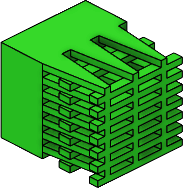
\includegraphics[height=\figheight]{sources-method-graded_lattice__green_only.png}
		\caption{Graded multi-stage ITIL}
		\label{interlocking:fig:graded_lattice}
	\end{subfigure}
	\begin{subfigure}[B]{.5\columnwidth}\centering
		
\includegraphics[height=\figheight]{sources-method-complex_interface__green_only.png}
		\caption{ITIL around spherical interface}
		\label{interlocking:fig:complex_interface_lattice}
	\end{subfigure}
	\caption{Extensions of ITIL. (Only PLA is shown.)}
	\label{interlocking:fig:lattice_interface}
\end{figure}


\subsection{Future work}
Future work might be aimed at loading scenarios different from tensile, different materials, different nozzle sizes and different layer heights.
Investigating other properties such as the displacement at break, stiffness or toughness would also be interesting under compressive loads.
It is specifically compelling to investigate the resilience of the interlocking structure against vertically applied loads.
\revise{}{If a larger space around the interface between the two bodies is allowed to be altered by the structure, one could optimize for a multi-layer interlocking structure, where the cells of the different layers have different geometry, such as visualized in \cref{interlocking:fig:graded_lattice}.}
Another interesting route is to optimize for an interface \revise{between two bodies }{}which has a complex geometry and heterogeneous stress distribution.
\revise{}{While the ITIL lattice inherently allows for complex interfaces (see \cref{interlocking:fig:complex_interface_lattice}), optimizing the orientation and geometry of cells for complex surfaces remains future work.}
In the light of sustainability and recycling one might select for specific failure modes, such as Z shear failure, which do not leave parts of the one material attached to the body of the other material after failure.
Taking a broader perspective one might design an interlocking structure which is both topologically interlocking and also has dovetail features.

\iffalse
If the design constraint on the length of the transitional structure between the two material is released,
the manufacturing constraints are less relevant, which means that the geometry of the structure is less restricted.
The geometry of the \revise{microstructure}{lattice}s could then be optimized for tailored mechanical properties.
In fact, such multi-material \revise{microstructure}{lattice}s could be tailored for functionally graded materials.
With a relatively large geometry of the functionally graded multi-material lattice structure,
the ITI\revise{M}{L} lattice can again be used to ensure connectivity between the two materials,
while the meso-scale structure could be used to guarantee the functionally graded mechanical properties.
\fi
